% LTeX: language=es
% !TEX program = xelatex
% !TEX options = --shell-escape -synctex=1 -interaction=nonstopmode -file-line-error "%DOC%"

\documentclass[aspectratio=169]{beamer}

\usepackage[spanish,es-noshorthands]{babel}
\usepackage{color}
\usepackage{xcolor}

\usepackage{enumerate}
\usepackage{booktabs, multirow} % for borders and merged ranges
\usepackage{soul}% for underlines
\usepackage{changepage,threeparttable}
\usepackage{float}
\usepackage{listings}
\usepackage{pdfpages}
\usepackage{minted}
\usepackage{multicol}
\usepackage{filecontents}

\usepackage{tikz}
\usetikzlibrary{shapes,arrows}

\newcount\mycount

%\graphicspath{{./}}

%\theoremstyle{definition}
%\newtheorem{definition}{Definici\'on}[section]
%\newtheorem{proposition}[definition]{Proposici\'on}
%\newtheorem{lemma}[definition]{Lema}
%\newtheorem{theorem}[definition]{Teorema}
%\newtheorem{corollary}[definition]{Corolario}
%\newtheorem{example}[definition]{Ejemplo}
%\newtheorem{observation}[definition]{Observaci\'on}
%\newtheorem{problem}{Problema}
%\newtheorem{question}[definition]{Pregunta}
\newtheorem{pointt}{}

\def\proof{\noindent{\textbf{Demostraci\'on}}\\}
\def\endproof{\hfill{\ensuremath\square}}
\def\refname{Referencias}
\allowdisplaybreaks



\usetheme{Boadilla}
\setbeamertemplate{blocks}[rounded][shadow=false]

\usefonttheme[onlymath]{serif}

\RequirePackage{fontspec}
%\setmainfont[Ligatures=TeX]{EB Garamond}
\setsansfont[Ligatures=TeX]{EBGaramond-VariableFont_wght.ttf}
%\setseriffont[Ligatures=TeX]{Raleway}
\newfontfamily\raleway{RalewayThin-wght350.ttf}
\newfontfamily\ebg{EBGaramond-VariableFont_wght.ttf}
%\newfontfamily{\semibold}{RalewayThin-Weight600}

\setmonofont{FiraCode-Regular.ttf}
%\usepackage{mathspec}
%\setmathrm{FiraCode-Regular.ttf}
%\setmathfont(Digits,Latin){FiraCode-Regular.ttf}
%\setmathfont[range=\mathit]{FiraCode-Regular.ttf}

\definecolor{backgroundColour}{RGB}{29, 29, 38}
\definecolor{textColour}{RGB}{179, 179, 212}
\definecolor{structureColour}{RGB}{255, 51, 153}
\definecolor{structure2Colour}{RGB}{204, 102, 255}
\definecolor{structure3Colour}{RGB}{255, 204, 102}
\setbeamercolor{normal text}{fg=textColour,bg=backgroundColour}
\setbeamercolor{structure}{fg=structureColour}

\setbeamercolor{palette primary}{use=structure,bg=structureColour, fg=textColour!50!white}
\setbeamercolor{palette secondary}{use=structure,bg=structureColour, fg=textColour!50!white}
\setbeamercolor{palette tertiary}{use=structure,bg=structureColour, fg=textColour!50!white}

\setbeamercolor{author}{fg=structure2Colour}
\setbeamercolor{subtitle}{fg=structure3Colour}
\setbeamercolor{alerted text}{fg=structure3Colour}
\setbeamercolor{highlighted}{fg=structure3Colour}

%\setbeamerfont{normal text}{family=\ebg}
%\setbeamerfont{structure}{family=\ebg}
%\setbeamerfont{block body}{family=\ebg}
\setbeamerfont{title}{size=\fontsize{18}{1},family=\raleway}
\setbeamerfont{frametitle}{size=\fontsize{18}{28},family=\raleway}



\title{Videojuegos e Inteligencia Artificial}

\author[Castro-Sotelo, García-Espinoza, Molina-Rebolledo] % (optional)
{C.A.~Castro-Sotelo \and A.T.~García-Espinoza \and I.~Molina-Rebolledo}

\institute[BUAP] % (optional)
{
  Facultad de Ciencias de la Computación\\
  Benemérita Universidad Autónoma de Puebla
}

\date[Otoño 2022] % (optional)
{Inteligencia Artificial, otoño 2022}



\date{14 de noviembre de 2022}
\def\code#1{\mintinline[fontsize=\small]{lean}{#1}}
%\beamerdefaultoverlayspecification{<+->}

\begin{document}
\frame{\titlepage}
%Highlighting text


\begin{frame}[fragile]
\frametitle{Videojuegos e Inteligencia Artificial}
\begin{columns}
\column{0.5\textwidth}
\begin{itemize}[<+->]
\item Cuando uno piensa en la inteligencia artificial en los videojuegos
  comúnmente se imagina la simulación de comportamientos de los personajes no
  manejados por el jugador.
\item La mayoría de videojuegos se trabajan con inteligencia artificial que
  permite que los personajes generados sean capaces de reaccionar según las
  circunstancias.
\end{itemize}
\column{0.5\textwidth}
\begin{center}
  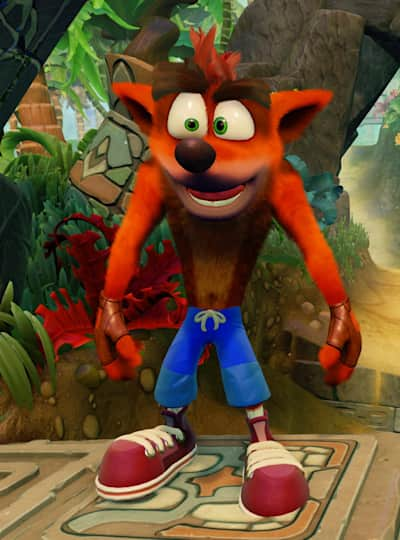
\includegraphics[width=0.4\textwidth]{./images/crash.jpg}
\end{center}
\end{columns}
\end{frame}

\begin{frame}
\frametitle{Videojuegos e Inteligencia Artificial}
\begin{columns}
\column{0.5\textwidth}
\begin{itemize}[<+->]
\item La inteligencia artificial también permite determinar el camino más corto
  que debe recorrer un personaje para ir entre el punto A y B, indica si está
  en peligro para huir o curarse aplicando algoritmos, entre otras
  aplicaciones.
\end{itemize}
\column{0.5\textwidth}
\begin{center}
  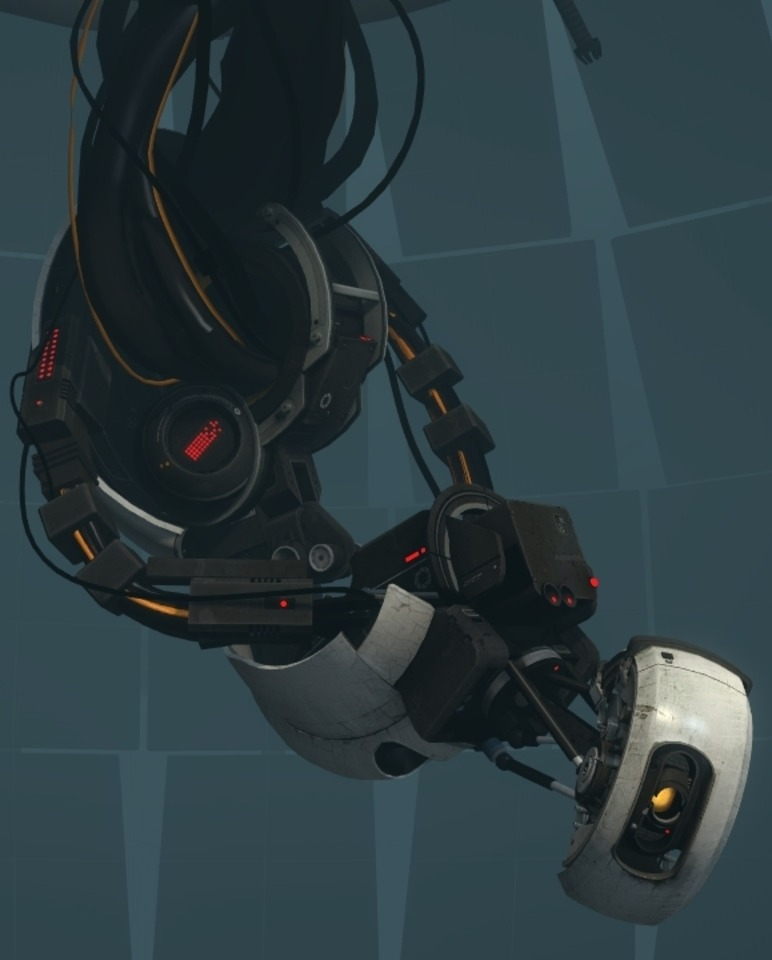
\includegraphics[width=0.4\textwidth]{./images/ai.jpeg}
\end{center}
\end{columns}
\end{frame}

\begin{frame}
\frametitle{Historia}
\begin{itemize}[<+->]
\item Fue los años 50 donde los primeros sistemas de inteligencia artificial se
  aplicaron a juegos de mesa: damas (Arthur Samuel) y ajedrez (Claude Shannon).
\item Para los años 60 se desarrollaron juegos como el Pong o Spacewar! basados
  en la lógica. 
\item En los 70 surgieron juegos de 1 jugador contra enemigos que se movían
  mediante patrones almacenados. 
\item En esta misma década, llegó Space Invaders (1978), el cual añadió
  dificultad creciente y respondía a las acciones del jugador.
\item En 1980, Pac-Man incorporó algoritmos de búsqueda en laberintos. 
\item Llegando a los años 90, surgió Dragon Warrior, el primer RPG que permitía
  variar las rutinas de la IA de los enemigos durante las batallas.
  \item Fue en esta década que se produjo un boom de nuevos géneros y nuevas
  técnicas de IA: máquinas de estados finitos, redes neuronales, computación
  evolutiva, lógica difusa, etc. Aquí tenemos a Battlecruiser 3000AD (1996)
  que incorpora redes neuronales.
\end{itemize}
\end{frame}

\begin{frame}
\begin{center}
La meta de la investigación en inteligencia artificial es inventar una
verdadera inteligencia artificial. En orden para construir una inteligencia
artificial completa necesitamos construir un sistema que tome acciones en un
tipo de ambiente.
\end{center}
\end{frame}

\begin{frame}
\begin{center}
Video.
\end{center}
\end{frame}

\begin{frame}
\frametitle{En la práctica...}
\begin{itemize}[<+->]
\item Una de las ideas más obvias para llevar esto a cabo sería incorporar una inteligencia artificial en robots.
\item La práctica, sin embargo, nos ha mostrado que incluso las tareas más mundanas son difíciles de realizar por robots. 
\item Trabajar con robots claramente tiene sus desventajas: son caros y lentos.
\item Un robot requeriría de mucho tiempo de entrenamiento y el desarrollo de pistas que prueben y desafíen el sistema en su toma de decisiones.
\end{itemize}
\end{frame}

\begin{frame}
\begin{center}
Es por esto que tomaremos la perspectiva de los videojuegos como pruebas de rendimiento para las inteligencias artificiales.
\end{center}
\end{frame}

% End of document
\begin{frame}
\frametitle{Final de la presentación}

Muchas gracias por su atención.
\end{frame}

\begin{frame}
\frametitle{Referencias}
\end{frame}

\end{document}
